\subsection{Conversion Manager [Simone]}
\label{sec:Insieme.Frontend.Convert}

\begin{figure}[tb]
	\centering
	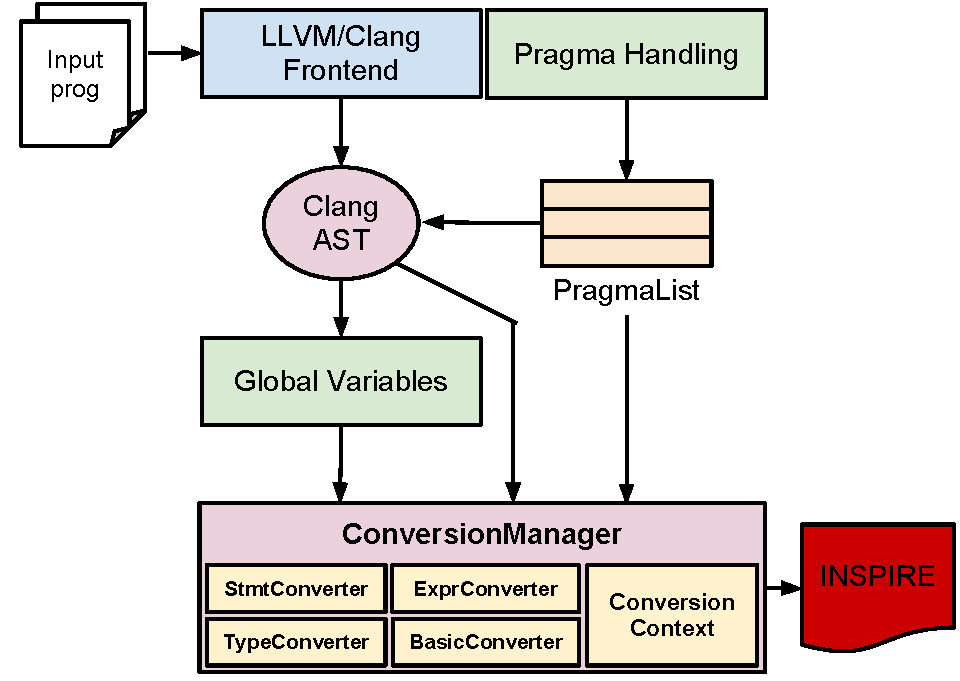
\includegraphics[width=0.8\textwidth]{compiler/frontend/seq_frontend.pdf}
	\caption{Dataflow of the Insieme Frontend}
	\label{fig:Frontend.Seq}
\end{figure}

In Figure~\ref{fig:Frontend.Seq}, the flow of execution of the frontend is
depicted. We already explained two component which are executed before the
actual conversion into IR is performed. The task of converting the {\tt
LLVM/Clang} AST is done by the \type{frontend::Conversion\-Manager}. In order
to reduce the complexity of the conversion procedure, we split the code into 4
"converters" taking care of specific aspects of the C language:

\begin{description}

\item [BasicConverter:] Defined in \file{frontend/basic\_convert.cpp}. It
contains utility functions which are used across all the converters.

\item [TypeConvert:]  Defined in \file{frontend/type\_convert.cpp}. It takes care
of the conversion of C/C++ types into IR types. 

\item [StmtConverter:] Defined in \file{frontend/stmt\_convert.cpp}. It takes care
of the conversion of C/C++ statements into IR statements. 

\item[ExprConverter:] Defined in \file{frontend/expr\_convert.cpp}. It takes care
of the conversion of C/C++ expressions into IR statements. 

\end{description}

To make the code readable, the implementation of the 4 converters are spread
across 4 translation units. Also, because of optimization issues related to the
amount of symbols being exported by the frontend {\tt .so} library, the
definition of those converters is completely hidden and not accessible outside
the frontend.  Because the \type{frontend::Con\-ver\-sion\-Manager} provides a facade
for invoking the conversion facility, so there is no need for external access of
the single converters. Communication among converters is obtained through the
manager class, this means that each converter can utilize functionalities of
another converter (or himself) through the \type{frontend::ConversionManager}
class whose interface is defined in \file{frontend/convert.h}.
Indeed the manager class provides 3 fundamental methods: 

\begin{description}
\item [{\tt TypePtr convertType(const clang::Type*)}:] Converts an {\tt
LLVM/Clang} type node into an INSIPRE type.

\item [{\tt ExpressionPtr convertExpr(const clang::Expr*)}:] Converts an
{\tt LLVM/Clang} expression node into an INSPIRE expression. 

\item [{\tt StatementPtr convertStmt(const clang::Stmt*)}:] Converts an
{\tt LLVM/Clang} statement node into an INSPIRE statement.

\end{description}

Beside taking care of dispatching the conversion task to the appropriate
converter, the manager also performs some optimizations at this stage in order
to speedup the conversion process. For example, by introducing caching we avoid
to convert symbols which have already been converted. Caching is not utilized
for all types of IR nodes as the probability of converting two identical
statements is very low. However, caching is quite successful for types nodes as
the type reference to type node ration is high. Future PhDs might be interested
in speeding up the frontend time and introducing smarter way of caching nodes
could be a simple and high effective way of doing it (low hanging fruit).

Finally, the manager also retains a context which stores information necessary
through the conversion process of the IR. In the context we store those
information which needs to be visible (or alive) during the conversion of the
entire program. For example, the mapping between a Clang variable declaration
and an IR variable makes sure the same C variable is being replaced by the same IR
entity consistently for all the encountered references to it. 

\subsubsection{Type Convert}
{\tt LLVM/Clang} supports a visitor interface for traversing the AST. For this
reason the class \type{frontend::TypeConverter} inherits from
\type{clang::TypeVisitor}. The visitor defines several methods which define how
the C AST node should be transformed into IR. Each method of the visitor returns
the generated node so that the IR representation of complex node can be built
upon composition of the type node returned by successive calls to the visitor
itself. 

One peculiarity of the \type{frontend::TypeConverter} is the way we deal with
pointers type. Indeed, the IR type system doesn't support the C semantics of
pointers which not necessary refers to the element directly pointed in memory.
For example, in C a pointer can be used to refer to an array of elements or a
singular scalar variables. Ideally the
following conversion semantics shall be used for pointer:

\begin{table}
\begin{centering}
	\begin{tabular}{l|c}
		\textbf{C Type} & \textbf{IR Type} \\
		\hline \hline
		\constant{type* (R-Value)}          & \insCodeInl{ref<'type>} \\
		\constant{type* (L-Value)} 		   & \insCodeInl{ref<ref<'type>} \\
		\hline 
	\end{tabular}
	\caption{Sound type conversions for C pointers}
	\label{tab:Compiler.Frontend.ml.GenNNoutput}
\end{centering}
\end{table}

However, because we must take into account situation for which the pointer is
used to refer to an array, and the user want to access a memory location which
is not at displacement 0, then a different encoding is necessary in order to
guarantee sound semantics check of the generated IR program. For these reason
the following encoding is utilized: 

\begin{table}
\begin{centering}
	\begin{tabular}{l|c}
		\textbf{C Type} & \textbf{IR Type} \\
		\hline \hline
		\constant{type* (R-Value)}          & \insCodeInl{ref<array<'type,1>>} \\
		\constant{type* (L-Value)} 		   & \insCodeInl{ref<ref<array<'type,1>>>} \\
		\hline 
	\end{tabular}
	\caption{Implemented type conversions for C pointers}
	\label{tab:Compiler.Frontend.ml.GenNNoutput}
\end{centering}
\end{table}

This however introduces several levels of ugliness to the IR code being
generated by the frontend. One way to really deal with this problem is to apply
a two phase approach which shall be implemented in Insieme. Because we don't
want to perform any advanced analysis on the input code, we let the frontend
produce an IR code which contains impurities (for example representing pointers
using IR arrays as it is now). Right after the frontend completes the
conversion, we may apply an analysis (on the generated IR) which data mine the
type of usage of pointers. If for example a pointer is always used to access the
element at displacement 0 then we can safely replace the IR type to be a
\insCodeInl{ref<'type>}. Those situations where the pointer is being used to
access elements with an offset not equal zero, then the array type should be
maintained. In those cases, DEF-USE \todo{ref DEF-USE} analysis may be used to
determine the declaration of the array being addressed and if possible replace
the \insCodeInl{ref<array<'type>>} with an actual
\insCodeInl{ref<vector<'type>>}. All of these are options which may be
implemented right after the first phase of the frontend has been processed. It
may improve both the readability of the generated IR code and possibility for
optimizations. \note{Proposal for 'array-erasure' procedure useful to cleanup
generated IR}.

